%\documentclass[11pt,a4paper,titlepage,twoside]{article}
\documentclass[12pt,a4paper,twoside]{article}
\usepackage{mystyle}
\usepackage{optik_v002}
\usepackage{foto_v001}
\usepackage{gplot}
%\usepackage{schueler}
%\usepackage{lehrer}
\date{}
%\author{Felix Binder}
\title{Optik}

%\usepackage{enumerate}

\newcommand{\Obox}{\draw (0,0) rectangle (\textwidth,0.7\textwidth);}




\begin{document}
\maketitle

Die Optik beschäftigt sich mit den Eigenschaften des Lichtes. Lichteffekte begegnen uns im täglichen Leben
überall. Man sieht etwas, das heisst Lichtstrahlen werden von einem Objekt reflektiert und fallen in unser Auge.
%Licht an glatten Oberflächen wird reflektiert. Beim Übergang von zwei verschieden Medien wird Licht gebrochen.

\section{Lichtquellen}

Es gibt sehr verschiedene Lichtquellen: Die Sonne, Kerzen, Lampen, der Fernseher und viele mehr.
Man unterscheidet zwischen drei verschiedenen Typen von Lichtquellen. Punktlichtquelle, Parallelstrahler und Flächenstrahler.

\begin{center}
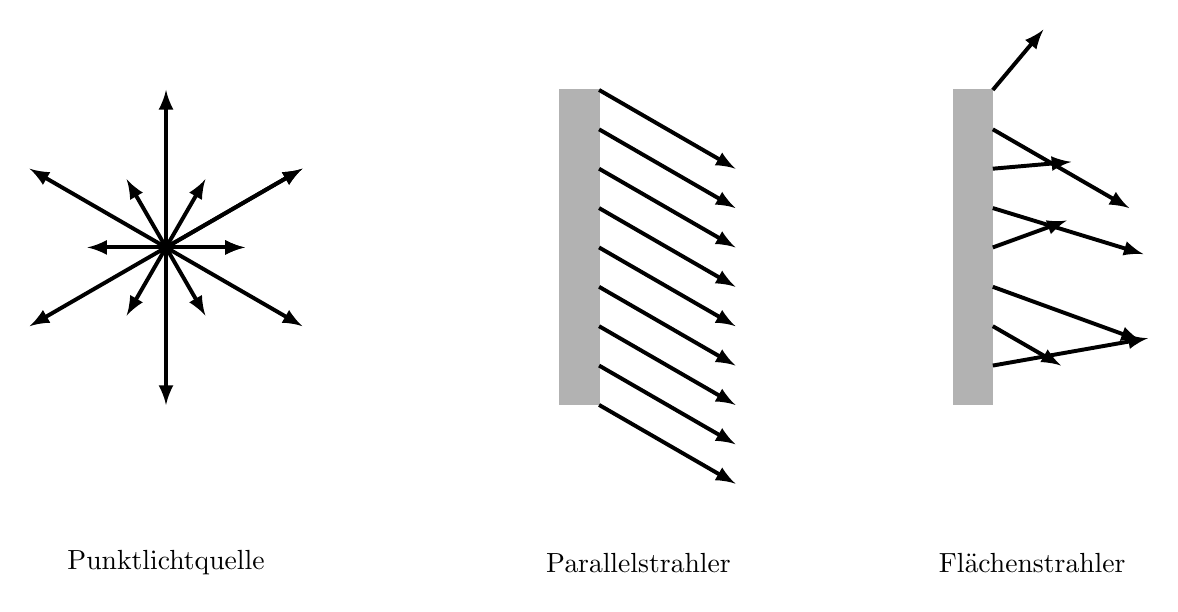
\begin{tikzpicture}
\tikzset{LS/.style={>=latex,line width=0.05cm}}

\node (Bezeichnung) at (0,-4cm) {Punktlichtquelle};
\foreach \x in {0,60,...,360}{
\draw[LS,->] (0,0) -- (\x:1cm);
\draw[LS,->] (0,0) -- ({\x+30}:2cm);
};


\def\XC{5cm}
\node (Bezeichnung) at ({\XC+1cm},-4cm) {Parallelstrahler};
\draw [fill,color=black!30](\XC,-2) rectangle ({\XC+0.5cm},2);
\foreach \y in {2,1.5,...,-2}{
\draw [LS,->]({\XC+0.5cm},\y) -- +(-30:2cm);
};

\def\XC{10cm}
\node (Bezeichnung) at ({\XC+1cm},-4cm) {Flächenstrahler};
\draw [fill,color=black!30](\XC,-2) rectangle ({\XC+0.5cm},2);
%\foreach \y in {2,1.5,...,-2}{
\draw [LS,->]({\XC+0.5cm},2) -- +(50:1cm);
\draw [LS,->]({\XC+0.5cm},1.5) -- +(-30:2cm);
\draw [LS,->]({\XC+0.5cm},1) -- +(5:1cm);
\draw [LS,->]({\XC+0.5cm},0.5) -- +(-17:2cm);
\draw [LS,->]({\XC+0.5cm},0) -- +(20:1cm);
\draw [LS,->]({\XC+0.5cm},-0.5) -- +(-20:2cm);
\draw [LS,->]({\XC+0.5cm},-1.0) -- +(-30:1cm);
\draw [LS,->]({\XC+0.5cm},-1.5) -- +(10:2cm);
%};
\end{tikzpicture}
\end{center}

\begin{aufgabe}
	Nennen Sie je drei Beispiele für eine Punktlichtquelle, einen Parallelstrahler und einen Flächenstrahler.
\end{aufgabe}

\vspace*{3cm}

Reale Lichtquellen kann man meistens nicht eindeutig diesen drei Grundtypen zuordnen. Als Beispiel wollen wir die
Sonne betrachten. Die Lichtstrahlen die auf der Erde ankommen sind nahezu parallel. Befindet man sich nahe der
Sonnenoberfläche, so ist die Sonne ein Flächenstrahler. Aus sehr grosser Entfernung ist unsere Sonne ein Stern,
also ein Punkt im dunklen Universum.

\section{Licht und Schatten}

\newcommand{\Schirm}[3]{\draw [DS] (#1)--(#2) node [rotate=90, above right] {#3};}
\newcommand{\SchirmR}[0]{\Schirm{INO}{ISO}{Schirm}}
%\newcommand{\SchirmR}[0]{\draw [DS] (INO)--(ISO) node [rotate=90, above right] {Schirm};}

%Schatten Punktlichtquelle
\begin{tikzpicture}
	\NObox
	\draw [fill] (0.1\textwidth,2) circle (0.1cm) node [above] {Lampe};
    \draw [OObjekt] (IO6) -- +(0,0.5cm) --+(0,-1cm) node [midway, rotate=90, above] {Objekt};
\SchirmR
\end{tikzpicture}

%Schatten Parallelstrahler
\begin{tikzpicture}
	\NObox
\foreach \x in{8,7.5,...,3}{
\draw [LS,->] (0.1\textwidth,\x)--+(-10:1cm);
};	
\draw (0.15\textwidth,1) node {Lichtrichtung}; 
    \draw [OObjekt] (IO6) -- +(0,0.5cm) --+(0,-1cm) node [midway, rotate=90, above] {Objekt};
    \draw [DS] (INO)--(ISO) node [rotate=90, above right] {Schirm};
\end{tikzpicture}

%Schatten Lampe 
\begin{tikzpicture}
	\NObox
%\foreach \x in{8,7.5,...,3}{
%\draw [LS,->] (0.1\textwidth,\x)--+(-10:1cm);
%};	
\draw [fill] (0.1\textwidth,4) rectangle (0.12\textwidth,6) node [above] {Lampe};
    \draw [OObjekt] (IO6) -- +(0,0.5cm) --+(0,-1cm) node [midway, rotate=90, above] {Objekt};
    \draw [DS] (INO)--(ISO) node [rotate=90, above right] {Schirm};
%\draw (0.15\textwidth,1) node {Lampe}; 
\end{tikzpicture}

\begin{aufgabe}
Eratosthenes (*276 v. Chr., $\dagger$ 194 v. Chr. in Alexandria) wusste, dass
	am 21.\ Juni zu Mittag die Sonne über Assuan genau im Zenit steht.
	Der Boden eines Brunnenschachtes wird vollständig von der Sonne beleuchtet. 
 Zur selben Zeit wirft ein Obelisk im nördlich von Assuan gelegenen Alexandria einen Schatten.
 Nimmt man die Sonnenstrahlen als parallel an, dann ist der Zenit etwa \SI{7.5}{\degree} entfernt.
 Daher muss der Brunnenschacht in Assuan mit dem Obelisken in Alekandrien wegen der
 Krümmung der Erdoberfläche einen Winkel von \SI{7.5}{\degree} einschliessen.
 Die Distanz zwischen Alexandria und Assuan beträgt etwa 5000 Stadien. Ein
 attisches Stadium beträgt \SI{185}{m}. Berechne Erdumfang und Erdradius.
\end{aufgabe}


\section{Bilder mit Licht und Schatten}
\begin{aufgabe}
	Konstruiere den Schlagschatten des Gegenstandes auf der Bildebene.

%Schatten Punktlichtquelle Pfeil
\begin{tikzpicture}
\NObox
\draw [->, LS] (0.6\textwidth,4)--(0.6\textwidth,6) node [above] {Gegenstand};
\SchirmR
	\draw [fill] (0.1\textwidth,2) circle (0.1cm) node [above] {Lampe};
\end{tikzpicture}

\begin{enumerate}[a)]
	\item Ist das Bild aufrecht oder verkehrt herum?
	\item Zeichne in der Figur die Grösse des Gegestandes $G$ und die Grösse des Bildes $B$ ein.
	\item Zeichne die Gegenstandsweite $g$ (Abstand Lampe\ --\ Gegenstand) und die Bildweite $b$
		(Abstand Lampe\ --\ Bild) ein.
	\item Um welchen Faktor wird das Bild im Vergleich zum Gegenstand vergrössert?
	\item Benutze $b$ und $g$ um die Vergrösserung auszudrücken.
\end{enumerate}
\end{aufgabe}


\newpage


\begin{aufgabe}
	Fragen zur Vergrösserung:
	\begin{enumerate}[a)]
		\item Wenn das Bild grösser als der Gegenstand ist, so ist der Zahlenwert der Vergrösserung \ldots.
		\item Wenn das Bild kleiner als der Gegenstand ist, so ist der Zahlenwert der Vergrösserung \ldots.
		\item Wird das Bild grösser oder kleiner, wenn man die Bildebene weiter von der Lampe entfernt?
		\item Wird das Bild grösser oder kleiner, wenn man den Gegenstand von der Lampe entfernt?
	\end{enumerate}
\end{aufgabe}

\section{Lochkamera}
\begin{aufgabe}
	Konstruiere das Bild des Gegenstandes auf dem Schirm.

%Lochkamera
\begin{tikzpicture}
\NObox
\draw [->, LS] (0.1\textwidth,4)--(0.1\textwidth,6) node [above] {Gegenstand};

\path (IO6) ++(-90:0.1cm) node (ENDE){};
\draw (IO6) ++(90:0.1cm) node [rotate=90, above] {}--(INO6)--(INO)--(ISO)--(ISO6) node [above, right] {}--(ENDE);

%\SchirmR
%\draw [DS] (0.6\textwidth,0.5)--(0.6\textwidth,5.2) (0.6\textwidth,5.3)--(0.6\textwidth,10) node [above] {Blende};
\end{tikzpicture}

\begin{enumerate}[a)]
	\item Ist das Bild aufrecht oder verkehrt herum?
	\item Zeichne in der Figur die Grösse des Gegestandes $G$ und die Grösse des Bildes $B$ ein.
	\item Zeichne die Gegenstandsweite $g$ (Abstand Gegenstand\ --\ Blende) und die Bildweite $b$
		(Abstand Blende\ --\ Bild) ein.
	\item Um welchen Faktor wird das Bild im Vergleich zum Gegenstand vergrössert?
	\item Benutze $b$ und $g$ um die Vergrösserung auszudrücken.
\end{enumerate}
\end{aufgabe}

\begin{aufgabe}
	Die Höhe eines Obelisken im Karnak-Tempel, \SI{2,5}{Kilometer} nördlich von Luxor, soll bestimmt werden.
	Ein zwei Meter langer Stab wirft einen Schatten von \SI{3,2}{Meter}. Der Schatten des Obelisken ist \SI{48}{Meter} lang.
	\begin{loesung}
		Der Stab und sein Schatten soll benutzt werden, um die Höhe des Obelisken zu bestimmen. Die Vergrösserung (der Abbildungsmassstab)
		von Stab und Schatten und Obelisk und dessen Schatten sind gleich gross, da die Sonne als Parallelstahler angesehen werden kann.
		\begin{eqnarray*}
			V=\frac{B}{G}=\frac{\SI{3.2}{m}}{\SI{2}{m}} = \num{1.6}
		\end{eqnarray*}
		Damit lässt sich die Höhe des Obelisken bestimmen:
		\begin{eqnarray*}
			V=\frac{B}{G}\to G=\frac{B}{V}=\frac{\SI{48}{m}}{\num{1.6}}=\SI{30}{m}\text{.}
		\end{eqnarray*}
	\end{loesung}
\end{aufgabe}

\begin{aufgabe}
	Beim Fingerschattenspiel werden Schatten, die von der Hand geformt werden an eine Leinwand projiziert.
	Als Lichtquelle dient eine Kerze. Sie soll \SI{25}{cm} von den Händen aufgestellt sein. Der Abstand von
	den Händen zur Wand soll \SI{90}{cm} betragen. Wie gross erscheint der Schattenriss des \SI{6.5}{cm} langen Daumen?
	\begin{loesung}
		Zum Lösen der Aufgabe ist eine Skizze empfehlenswert.
		\begin{eqnarray*}
			V=\frac{b}{g}=\frac{\SI{90}{cm}}{\SI{25}{cm}}=\num{3.6}
		\end{eqnarray*}
		\begin{eqnarray*}
			V=\frac{B}{G}\to B=V\cdot G = \num{3.6}\cdot\SI{6.5}{cm}=\SI{23.4}{cm}\text{.}
		\end{eqnarray*}
	\end{loesung}
\end{aufgabe}

\begin{aufgabe}
	Die Rückseite einer Lochkamera der Firma Kodak aus dem Jahre 1930 ist \SI{4.25}{''} von der Blende entfernt.
	Eine \SI{12}{cm} grosse Kerze ist \SI{50}{cm} von der Kamera entfernt. Wie gross ist die Kerze auf dem Filmnegativ?
	Wie ist die Vergrösserung?
	\begin{loesung}
		Zum Lösen der Aufgabe ist eine Skizze empfehlenswert.
		Die Bildweite ist $b=\SI{4.25}{''}=\SI{10.8}{cm}$.
		\begin{eqnarray*}
			V=\frac{b}{g}=\frac{\SI{10.8}{cm}}{\SI{50}{cm}}=\num{0.22}
		\end{eqnarray*}
		\begin{eqnarray*}
			V=\frac{B}{G}\to B=V\cdot G = \num{0.22}\cdot\SI{12}{cm}=\SI{2.59}{cm}\text{.}
		\end{eqnarray*}
	\end{loesung}
\end{aufgabe}

\begin{aufgabe}
	Der Bildsensor einer digitalen Spiegelreflexkamera ist \SI{22,2}{mm} breit und \SI{14,8}{mm} hoch.
	Das Auflagemass, das ist der Abstand vom Bildsensor zum Objektivgewinde ist \SI{44}{mm}.
	Schraubt man auf das Objektivgewinde eine Lochblende, steht diese weiter \SI{5}{mm} hervor.
	In welcher Entfernung zur Kamera muss eine \SI{1,70}{m} grosse Person mindestens stehen, um vollständig auf einem Foto zu erscheinen?
	\begin{loesung}
		Zum Lösen der Aufgabe ist eine Skizze empfehlenswert.
		Die Bildweite ist $b=\SI{44}{mm}+\SI{5}{mm}=\SI{49}{mm}$.
		\begin{eqnarray*}
			V=\frac{B}{G}=\frac{\SI{14.8}{mm}}{\SI{1.7}{m}}=\num{0.0087}
		\end{eqnarray*}
		\begin{eqnarray*}
			V=\frac{b}{g}\to g=\frac{b}{V}=\frac{\SI{49}{mm}}{\num{0.0087}}=\SI{5628.4}{mm} \approx\SI{5.63}{m}
		\end{eqnarray*}
	\end{loesung}
\end{aufgabe}

\newpage
\section{Reflexion und Streuung}


\begin{aufgabe}
Zeichnen Sie den Lichtstahl, der von der Lampe kommt weiter. Was passiert, wenn der Lichtstrahl auf den Spiegel trifft?	

%Spiegel
\begin{tikzpicture}
\NObox
\draw [fill] (0.1\textwidth,4) circle (0.125cm) node [above] {Lampe};
\draw [->, LS] (0.1\textwidth,4)--+(-53:2cm);
\draw [DS] (0.1\textwidth,0.5)--(0.9\textwidth,0.5) node [above] {Spiegel};
\end{tikzpicture}
\end{aufgabe}

\begin{aufgabe}
	Mit einem Spiegel kann man die Höhe eines Baumes bestimmen. Wollen Sie die Höhe eines besonders hohen Baumes bestimmen,
	so legen Sie einen kleinen Spiegel \SI{40}{m} von diesem Baum entfernt. Entfernen Sie sich vom Spiegel, bis Sie die
	Spitze des Baumes im Spiegel erkennen. Sie sind nun \SI{2}{m} vom Spiegel entfernt. Ihre Augen sind \SI{1.6}{m} über dem Boden.
	Wie hoch ist der Baum?
\end{aufgabe}

\begin{minipage}{0.5\textwidth}
\begin{aufgabe}
	Die Skizze zeigt den Aufbau eines Periskops. Dies wird z.B. in U-Booten benutzt. Ist das Bild, dass du beim Hindurchschauen
	durch das Periskop siehst aufrecht oder steht es auf dem Kopf?
\end{aufgabe}
\end{minipage}
\begin{minipage}{0.5\textwidth}
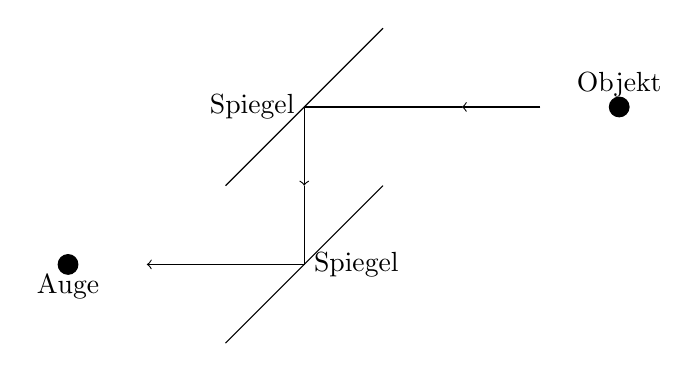
\begin{tikzpicture}

\draw (0,0)--(2,2) node [midway, left] {Spiegel};
\draw (0,-2)--(2,0) node [midway,right] {Spiegel};

\draw [->] (4,1)--(3,1); 
\draw [->] (3,1)--(1,1)--(1,0);
\draw [->] (1,0)--(1,-1)--(-1,-1);

\draw [fill] (-2,-1) circle(0.125) node [below] {Auge};
\draw [fill] (5,1) circle(0.125) node [above] {Objekt};
\end{tikzpicture}

\end{minipage}

\newpage

\begin{aufgabe}
Erinnern Sie sich an Spiegelungen in der Mathematik? Zeichnen Sie den Strahlengang vom Objekt zum Auge ein, ohne einen Winkel zu messen.\\	
%Spiegel
\begin{tikzpicture}
\NObox
\draw [fill] (0.23\textwidth,2.5) circle (0.125cm) node [left] {Auge};
\draw [fill] (0.1\textwidth,8) circle (0.125cm) node [left] {Objekt};

\Schirm{IN}{IS}{Spiegel}
\end{tikzpicture}
\end{aufgabe}

\begin{aufgabe}
	In der Figur unten ist ein Spiegel zu sehen, der aus mehreren Elementen besteht, die in einem Winkel von \SI{90}{\degree}
	angeordnet sind. Zeichnen Sie den einfallenden Lichtstrahl weiter. Was gilt für den reflektierten Lichtstrahl?

%Spiegel mit 90Grad Winkel
\begin{tikzpicture}
\NObox
\draw [fill] (IO1) circle (0.125cm) node [above] {Lampe};
\draw [->, LS] (IO1)--+(-11:6cm);
\draw [DS] (0.9\textwidth,9.5)--++(-135:4cm)--++(-45:4cm)--++(-135:4cm) node [midway, right] {Spiegel};
\end{tikzpicture}

\end{aufgabe}


Tritt ein Lichtstrahl auf eine raue Oberfläche auf, wird er in verschiedene Richtungen abgelenkt. Dies Art der diffusen Reflexion
nennt man Streuung.

%raue Oberfläche
\begin{tikzpicture}
\NObox
\foreach \x in {0.15,0.25,...,0.95}{
\draw [->, LS] (\x\textwidth,10)--+(-90:2cm);
};
\draw [DS] (0.1\textwidth,0.5)--++(-11:1cm)--++(13:1.2cm)--++(88:1cm)--++(-20:2cm)--++(70:2.5cm)--++(-55:1cm)--++(17:2.2cm)--++(-49:0.8cm)--++(-30:1cm)--++(75:1cm)--++(-88:2cm)--++(5:1cm)--++(-35:1.7cm)--++(40:1.2cm) node [above] {Spiegel};
\end{tikzpicture}

\newpage

\section{Gewölbte Spiegel}
Im folgenden wollen wir das Reflexionsgesetz für gewölbten Spiegel anwenden. 
\begin{aufgabe}
Überlegen Sie, wie die parallel einfallenden
Lichtstrahlen am Hohlspiegel (konkaver Spiegel) reflektiert werden.

\begin{center}
\begin{tikzpicture}
\NObox

\HSpiegel{IO}{3}

\foreach \y in {-2,-1,...,2}{
\draw [LS,->] ($(IW) - (0,\y)$)--++(0:2cm);
}


\end{tikzpicture}
\end{center}
\end{aufgabe}

\newpage


%\begin{aufgabe}
%Überlegen Sie, wie die parallel einfallenden
%Lichtstrahlen am Wölbspiegel (konvexer Spiegel) reflektiert werden.

\begin{center}
	\begin{tikzpicture}[rotate=90]
\NObox
\draw (NW) node [transform shape,text width=15cm,above right]{%
\begin{aufgabe}
Überlegen Sie, wie die parallel einfallenden
Lichtstrahlen am Wölbspiegel (konvexer Spiegel) reflektiert werden.
\end{aufgabe}};

\WSpiegel{IO9}{3}

\foreach \y in {-2,-1,...,2}{
\draw [LS,->] ($(IW) - (0,\y)$)--++(0:2cm);
}


\end{tikzpicture}
\end{center}
%\end{aufgabe}

\newpage
\subsection{Abbildungen mit gewölbten Spiegeln}
\begin{aufgabe}
	Betrachten Sie sich in einem Hohlspiegel. Was sehen Sie? Ist das Bild abhängig vom Abstand zum Spiegel?
\end{aufgabe}

%Objekt ausserhalb des Kreispittelpunktes
\subsection*{$g>2\cdot f$}
\begin{center}
	\begin{tikzpicture}
		\AbbHS{IO3}
	\end{tikzpicture}
\end{center}

%Objekt im Mittelpunkt des Kreises
\subsection*{$g=2\cdot f$}
\begin{center}
	\begin{tikzpicture}
		\AbbHS{Spiegel C}
	\end{tikzpicture}
\end{center}

%Objekt zwischen Mittelpunkt und Brennpunkt
\subsection*{$g<2\cdot f$ und $g>f$}
\begin{center}
	\begin{tikzpicture}
		\path (Spiegel C) -- (Spiegel F) node [pos=0.5, shape=coordinate] (M1) {};
		\AbbHS{M1}
	\end{tikzpicture}
\end{center}

%Objekt im Brennpunkt
\subsection*{$g=f$}
\begin{center}
	\begin{tikzpicture}
		\AbbHS{Spiegel F}
	\end{tikzpicture}
\end{center}

%Objekt zwischen Brennpunkt und Spiegel
\subsection*{$g<f$}
\begin{center}
	\begin{tikzpicture}
		\path (Spiegel F) -- (IO) node [pos=0.5, shape=coordinate] (M1) {};
		\AbbHS{M1}
	\end{tikzpicture}
\end{center}



\begin{loesung}

%Objekt ausserhalb des Kreispittelpunktes
\subsection*{$g>2\cdot f$}
\begin{center}
	\begin{tikzpicture}
		\AbbHSLoesung{IO3}
	\end{tikzpicture}
\end{center}

%Objekt im Mittelpunkt des Kreises
\subsection*{$g=2\cdot f$}
\begin{center}
	\begin{tikzpicture}
		\AbbHSLoesung{Spiegel C}
	\end{tikzpicture}
\end{center}

%Objekt zwischen Mittelpunkt und Brennpunkt
\subsection*{$g<2\cdot f$ und $g>f$}
\begin{center}
	\begin{tikzpicture}
		\path (Spiegel C) -- (Spiegel F) node [pos=0.5, shape=coordinate] (M1) {};
		\AbbHSLoesung{M1}
	\end{tikzpicture}
\end{center}

%Objekt im Brennpunkt
\subsection*{$g=f$}
\begin{center}
	\begin{tikzpicture}
		\AbbHS{Spiegel F}
		\AbbHSLoesung{Spiegel F}
	\end{tikzpicture}
\end{center}

%Objekt zwischen Brennpunkt und Spiegel
\subsection*{$g<f$}
\begin{center}
	\begin{tikzpicture}
		\path (Spiegel F) -- (IO) node [pos=0.5, shape=coordinate] (M1) {};
		\AbbHSLoesung{M1}
	\end{tikzpicture}
\end{center}


\end{loesung}


\newpage
\section{Brechung}

\begin{minipage}{0.5\textwidth}
\begin{aufgabe}
	Zum Splitterschutz werden Fensterscheiben auf der Innenseite oft mit einer Plastikfolie versehen.
	Plastikfolie ist optisch dünner als Fensterglas.
	\begin{enumerate} [a)]
		\item Verlängere den eingezeichneten Lichtstrahl, so dass er einmal durch die gesamte Fensterscheibe geht.
		\item Erscheint die Umgebung beim betrachten durch die Scheibe verzerrt?
	\end{enumerate}
\end{aufgabe}
\end{minipage}
\begin{minipage}{0.5\textwidth}
	\begin{center}
	\begin{tikzpicture}
\draw (0,0) -- (5,0) node [above] {Aussenluft};
\draw (0,-1)--(5,-1) node [above]{Fensterglas};
\draw (0,-2)--(5,-2) node [above]{Plastikfolie};
\draw (0,-3) -- (5,-3) node [above] {Innenluft};

\draw [LS,<-](1,0)--+(150:1cm);

\end{tikzpicture}
	\end{center}
\end{minipage}

\begin{aufgabe}
	Ein Lichtstrahl trifft auf eine Wasseroberfläche. Der Einfallswinkel beträgt \SI{30}{\degree}. Wie gross ist der Brechungswinkel?
	\begin{loesung}
		Es ist nützlich eine Skizze zu machen.
		\begin{eqnarray*}
			n_1\cdot\sin\alpha_1 = n_2\cdot\sin\alpha_2 \to \sin\alpha_2=\frac{\sin\alpha_1}{n_2}=\frac{\sin\SI{30}{\degree}}{\num{1.333}}=\num{0.375}
		\end{eqnarray*}
		Damit ist der Brechungswinkel etwa \SI{22}{\degree}.
	\end{loesung}
\end{aufgabe}

\begin{aufgabe}
	Ein Lichtstrahl trifft aus der Luft unter einem Einfallswinkel von \SI{72}{\degree} auf eine Diamantenoberfläche.
	Wie gross ist der Brechungswinkel?
\end{aufgabe}

\Spalten{0.5}{
\begin{aufgabe}
Bestimmen Sie die Brechungswinkel für den Übergang von Wasser zu Luft für die Winkel:
\SI{10}{\degree}, \SI{20}{\degree}, \SI{30}{\degree}, \SI{40}{\degree}, \SI{45}{\degree} und \SI{50}{\degree}
und zeichnen Sie die Lichtstrahlen in der Zeichnung weiter.  
\end{aufgabe}
}{0.5}{
\begin{center}
\begin{tikzpicture}
\fill [color=blue!20] (0,0) rectangle (5,-5);
\fill [color=white] (0,0) rectangle (5,5);
%
\draw (0,0) node [above right] {Luft} -- (5,0);
\draw (0,0) node [below right] {Wasser}-- (5,0);

\draw [LS,->](4,-4)--+(80:1cm);
\draw [LS,->](3,-4)--+(70:1cm);
\draw [LS,->](2,-4)--+(60:1cm);
\draw [LS,->](1,-4)--+(50:1cm);
\draw [LS,->](0.5,-3)--+(45:1cm);
\draw [LS,->](0.5,-2)--+(40:1cm);
\end{tikzpicture}
\end{center}
}

\begin{loesung}
		Es ist nützlich eine Skizze zu machen.
		\begin{eqnarray*}
			n_1\cdot\sin\alpha_1 = n_2\cdot\sin\alpha_2 \to \sin\alpha_2=\frac{\sin\alpha_1}{n_2}=\frac{\num{1.333}\cdot\sin\SI{10}{\degree}}{1}=\num{0.23}
		\end{eqnarray*}
		Einfallswinkel \SI{10}{\degree} Brechungswinkel etwa \SI{13}{\degree}.\\
		Einfallswinkel \SI{20}{\degree} Brechungswinkel etwa \SI{27}{\degree}.\\
		Einfallswinkel \SI{30}{\degree} Brechungswinkel etwa \SI{42}{\degree}.\\
		Einfallswinkel \SI{40}{\degree} Brechungswinkel etwa \SI{59}{\degree}.\\
		Einfallswinkel \SI{45}{\degree} Brechungswinkel etwa \SI{70}{\degree}.\\
		Einfallswinkel \SI{50}{\degree} hier gibt es keinen Brechungswinkel.
\end{loesung}

\begin{aufgabe}
Wie gross ist der Grenzwinkel für Totalreflexion beim Übergang zwischen Wasser und Luft?
Wie gross ist er für den Übergang Diamant - Luft und für den Übergang Diamant - Wasser?	
\begin{loesung}
	Es gilt das Brechungsgesetz. Wenn ein Lichtstrahl aus einem optisch dichteren in ein optisch dünneres Material wechselt,
	dann wird der Lichtstrahl vom Lot weg gebrochen. Das heisst, der Brechungswinkel ist grösser als der Einfallswinkel.
	Zur Totalreflexion kommt es, wenn der Brechungswinkel gleich \SI{90}{\degree} ist.
		\begin{eqnarray*}
			n_1\cdot\sin\alpha_1 = n_2\cdot\sin\alpha_2 \to \sin\alpha_1=\frac{n_2}{n_1}\cdot\sin\alpha_2=\frac{n_2}{n_1}\cdot\sin\SI{90}{\degree}=\frac{n_2}{n_1}
		\end{eqnarray*}
		Nun können wir die einzelnen Fälle untersuchen:\\
		Wasser -- Luft: $\sin\alpha_1=\frac{n_2}{n_1}=\frac{1}{\num{1.333}} \to \alpha_1=\SI{48.6}{\degree}$\\
		Diamant -- Luft: $\sin\alpha_1=\frac{n_2}{n_1}=\frac{1}{\num{2.}} \to \alpha_1=\SI{48.6}{\degree}$\\
		Diamant -- Wasser: $\sin\alpha_1=\frac{n_2}{n_1}=\frac{1.333}{\num{2.}} \to \alpha_1=\SI{48.6}{\degree}$\\\\

\end{loesung}
\end{aufgabe}




\begin{aufgabe}
Diamant hat eine hohe optische Dichte. Dadurch ist der Grenzwinkel für totale Reflexion
beim Übergang Diamant--Luft klein.
Dies bewirkt, dass einmal vom Diamanten ``eingefangenes'' Licht nur schlecht wieder den Diamanten verlässt.
Der Diamant funkelt.
\begin{itemize}
	\item [a)] Wie gross ist der Grenzwinkel der Totalreflexion für Diamant und Luft?
	\item [b)] Zeichnen Sie den Strahlengang durch die folgenden Diamanten und geben Sie alle Winkel an.
		\begin{center}
			
\begin{tikzpicture}
\draw [line width=0.05cm] (0,0)--+(0:5cm)--++(60:5cm)--cycle;
\draw [LS,->] (1,-2)--(1,0);
\end{tikzpicture}

\vspace*{1cm}

\begin{tikzpicture}
\draw [line width=0.05cm] (0,0) rectangle (5,5);
\draw [LS,<-] (2.5,0)--+(-45:2cm);

\draw [<->=latex, line width=0.05cm] (4,0) arc (0:-45:1.5cm);
\path (4,0) arc (0:-22.5:1cm) node [left] {$\SI{45}{\degree}$};

\end{tikzpicture}
		\end{center}


\end{itemize}
\end{aufgabe}







\section{Linsen}

Optische Linsen sind aus lichtdurlässigen Materialien, wie Glas oder Plastik, manchmal auch aus durchsichtigen Kristallen.
Einfache (sphärische) Linsen kann man sich aus einer Kugel geschnitten vorstellen. Der Kugelradius kann dabei verschieden gross sein.
Beim Durchlauf des Lichtstrahl durch die Linse, passiert er zwei Grenzflächen, an denen er nach dem Brechungsgesetz gebrochen wird.

\begin{aufgabe}
Zeichnen Sie den vollständigen Strahlengang für mindestens zwei parallel einlaufende Lichtstrahlen.
Die optische Dichte der Linse ist \num{1.5}.
\end{aufgabe}

\begin{center}
\begin{tikzpicture}
	\draw [mmPapier, xstep=0.5, ystep=0.5, shift={(-7,-5)}](0,0) grid (14,10);
	\def\RI{8}
	\def\RII{7}
	\Linse{(0,0)}{\RI}{\RII}{4}{0}{Lin}{Glas}

	%Mittelpunkte
	\draw [fill] (Lin Cl) circle(0.1cm) node [below] {C};
	\draw [dotted] (Lin POSr) arc (0:90:\RI);
	\draw [dotted] (Lin POSr) arc (0:-90:\RI);
	\draw [LS,->] (Lin Cl) --+(65:\RI) node [above, sloped, midway] {$R_1$};
	
	\draw [fill] (Lin Cr) circle(0.1cm) node [below] {C};
	\draw [dotted] (Lin POSl) arc (180:90:\RII);
	\draw [dotted] (Lin POSl) arc (180:270:\RII);
	\draw [LS,->] (Lin Cr) --+(125:\RII) node [above, sloped, midway] {$R_2$};

	
	\draw [dotted] (Lin POSo) -- (Lin POSu);
	\draw [dotted] (-7,0)--(7,0);
\end{tikzpicture}
\end{center}


Linsen werden in sehr vielen optischen Geräten verwendet. Um deren Funktionsweise verstehen zu können, ist es meistens nicht
nötig den genauen Stahlengang eines Lichtstrahl durch die Linse zu kennen. Für technische Anwendungen, und auch für unseren weiteren
Unterricht, läuft ein parallel zur optischen Achse einlaufender Lichtstrahl, bis zur \emph{Mittelebene} der Linse, und wird erst dort gebrochen.

\begin{aufgabe}
	Zeichnen Sie den Strahlengang für einen parallel zur optischen Achse einlaufenden Lichtstrahl, für einen Lichtstrahl, der durch
	den Brennpunkt auf die Linse fällt und für einen Lichtstrahl, der durch den Mittelpunkt der Linse verläuft.
\end{aufgabe}

\begin{center}
\begin{tikzpicture}
%	\draw [mmPapier, xstep=0.5, ystep=0.5, shift={(-7,-5)}](0,0) grid (14,10);
	\def\RI{12}
	\def\RII{12}
	\Linse{(0,0)}{\RI}{\RII}{4}{0}{Lin}{Glas}

	%Mittelpunkte
	\draw [fill] (-5,0) circle(\BPunkt) node [below] {F};
	
	\draw [fill] (5,0) circle(\BPunkt) node [below] {F};

	
	\draw [dotted] (Lin POSo) -- (Lin POSu);
	\draw [dotted] (-7,0)--(7,0);
\end{tikzpicture}
\end{center}

\begin{aufgabe}
	Zeichnen Sie den Strahlengang für parallel zur optischen Achse einlaufende Lichtstrahlen ein.
\end{aufgabe}

\begin{center}
\begin{tikzpicture}
%	\draw [mmPapier, xstep=0.5, ystep=0.5, shift={(-7,-5)}](0,0) grid (14,10);
	\def\RI{-12}
	\def\RII{-12}
	\Linse{(0,0)}{\RI}{\RII}{4}{2}{Lin}{Glas}

	%Mittelpunkte
	\draw [fill] (-5,0) circle(\BPunkt) node [below] {F};
	
	\draw [fill] (5,0) circle(\BPunkt) node [below] {F};

	
	\draw [dotted] (Lin POSo) -- (Lin POSu);
	\draw [dotted] (-7,0)--(7,0);
\end{tikzpicture}
\end{center}

\newpage
\section{Abbildungen mit Linsen}
Eine Linse kann einen Gegenstand abbilden. Die Konstruktion verläuft sehr ähnlich
wie bei der Abbildung am gewölbten Spiegel. Wir zeichnen jeweils den Parallelstahl,
den Brennpunktstrahl und den Mittelpunktstahl von der Spitze des Gegenstands ein.

\begin{tikzpicture}
\NObox
	\Biconvex{(IO5)}{Lin}
	\draw [OAchse] (IW)--(IO);
	\draw [OAchse] (IN)--(IS);
	\BP{(IO3)}
	\BP{(IO7)}
	\OG{(IW)}
\end{tikzpicture}


Aus geometrischen Überlegungen kann man für dünne Linsen eine Formel finden,
die die Brennweite $f$, die Bildweite $b$ und die Gegenstandsweite $g$ miteinander
in Beziehung setzt. Es gilt
\begin{eqnarray*}
	\frac{1}{f} = \frac{1}{b} + \frac{1}{g}\text{.}
\end{eqnarray*}

Zwischen der Grösse des Bildes $B$ und der Grösse des Gegenstandes $G$ gilt das selbe Verhältnis,
wie wir es auch schon bei anderen Abbildungen gesehen haben
\begin{eqnarray*}
	A = \frac{B}{G} = \frac{b}{g}\text{.}
\end{eqnarray*}

\begin{aufgabe}
	Die Sammellinse eines Diaprojektors hat eine Brennweite von \SI{10}{cm}. Ein Dia ($G=\SI{36}{mm}$)
	soll auf die Leinwand, die \SI{2.5}{m} von der Linse entfernt ist, abgebildet werden.
	\begin{enumerate} [a)]
		\item Wie weit ist die Linse vom Dia entfernt?
		\item Wie gross ist das Bild auf der Leinwand?
	\end{enumerate}
\end{aufgabe}

\subsection*{$g=2\cdot f$}
\begin{tikzpicture}
\NObox
	\Biconvex{(IO5)}{Lin}
	\draw [OAchse] (IW)--(IO);
	\draw [OAchse] (IN)--(IS);
	\BP{(IO3)}
	\BP{(IO7)}
	\OG{(IO1)}
\end{tikzpicture}

\subsection*{$g>f$ und $g<2\cdot f$}
\begin{tikzpicture}
\NObox
	\Biconvex{(IO5)}{Lin}
	\draw [OAchse] (IW)--(IO);
	\draw [OAchse] (IN)--(IS);
	\BP{(IO3)}
	\BP{(IO7)}
	\OG{(IO2)}
\end{tikzpicture}

\subsection*{$g=f$}
\begin{tikzpicture}
\NObox
	\Biconvex{(IO5)}{Lin}
	\draw [OAchse] (IW)--(IO);
	\draw [OAchse] (IN)--(IS);
	\BP{(IO3)}
	\BP{(IO7)}
	\OG{(IO3)}
\end{tikzpicture}

\subsection*{$g<f$}
\begin{tikzpicture}
\NObox
	\Biconvex{(IO5)}{Lin}
	\draw [OAchse] (IW)--(IO);
	\draw [OAchse] (IN)--(IS);
	\BP{(IO3)}
	\BP{(IO7)}
	\OG{(IO4)}
\end{tikzpicture}


\newpage

\section{Optische Geräte}

\subsection{Das menschliche Auge}
%\import{./Eye_scheme.pdf}{./Eye_scheme.pdf_tex}
\begin{center}
\Bildeinbinden{Eye_scheme2.pdf}{0.65\textwidth}
\end{center}

Licht tritt durch die Pupille ins Auge ein. Der Durchmesser der Pupille ist veränderlich. Ist es sehr hell verengt sich die Pupille,
ist es dunkel öffnet sich die Pupille, dadurch kann mehr Licht in das Auge eindringen. Beim Fotoapparat erfüllt die Blende die Funktion der Pupille. 

Die Netzhaut ist eine dünne lichtempfindliche Schicht aus Nervenzellen. Es gibt zwei verschiedene Typen von Nervenzellen auf der Netzhaut,
die Stäbchen und die Zäpfchen. Die Zäpfchen können verschiedene Farben unterscheiden, während die Stäbchen nur zwischen hell und dunkel unterscheiden können.
Ist es dunkel sprechen nur die Stäbchen an, und man kann keine Farben erkennen.

Die Form der Augenlinse, und damit auch die Brennweite der Linse, lässt sich durch die Ziliarkörper etwas verändern.
Befindet sich ein Gegenstand nah am Auge, dann vergrössert der Zilarkörper die Krümmung der Linse, dadurch verringert sich die Brennweite der Linse, und
die Strahlen vom Gegenstand werden wieder auf die Netzhaut fokussiert.
Befindet sich ein Gegenstand zu nah am Auge, kann dieses den Gegenstand nicht mehr scharf auf der Netzhaut abbilden.
Der minimale Abstand, bei dem ein Gegenstand noch scharf dargestellt werden kann heisst Nahpunkt.
Der Nahpunkt kann von Mensch zu Mensch verschieden sein, und ändert sich auch im Laufe des Lebens.
Als Standardwert gilt ein Nahbereich von \SI{25}{Zentimetern}.

\begin{aufgabe}
	Bestimmen Sie (am besten zu zweit) ihren persönlichen Nahpunkt.
	\begin{loesung}
		Der Nahpunkt variiert von Person zu Person, und kann zwischen 10 und \SI{200}{Zentimetern} liegen.
Als Standardwert gilt ein Nahbereich von \SI{25}{Zentimetern}.
	\end{loesung}
\end{aufgabe}
\begin{aufgabe}
	In welchem Bereich liegt die Brennweite des menschlichen Auges. Der Abstand Netzhaut--Linse soll \SI{2.5}{Zentimeter} betragen.
	\begin{loesung}
		Ist ein Gegenstand weit entfernt ($g=\infty$), dann ist die Augenlinse beim Betrachten entspannt.
		Aus der Linsengleichung wird in diesem Fall ($\nicefrac{1}{g}\to 0$)
		\begin{eqnarray*}
			\frac{1}{f}=\frac{1}{b}=\frac{1}{\SI{2.5}{cm}}\text{.}
		\end{eqnarray*}
		Die Brennweite ist dann also \SI{2.5}{cm}.

		Ist der Gegenstand nah am Auge, hier $g=\SI{25}{cm}$, dann gilt
		\begin{eqnarray*}
			\frac{1}{f}=\frac{1}{b} + \frac{1}{g} =\frac{1}{\SI{2.5}{cm}} + \frac{1}{\SI{25}{cm}}=\SI{0.4}{cm^{-1}} + \SI{0.04}{cm^{-1}}=\SI{0.44}{cm^{-1}}\text{.}
		\end{eqnarray*}
		Damit ist die Brennweite für diesen Fall $f=\SI{2.27}{cm}$.
	\end{loesung}
\end{aufgabe}

\subsection{Sehwinkel und Auflösung des Auges}
Lichtstrahlen, die von einem Gegenstand ausgehen fallen unter einem bestimmten Winkel, dem \emph{Sehwinkel} in unser Auge.
Ist der Gegenstand nah, so ist der Sehwinkel gross. Entfernt man den Gegenstand, wird der Sehwinkel kleiner.
Je nach Grösse des Sehwinkels erscheint uns der Gegenstand gross oder klein.

\begin{aufgabe}
	Messen Sie mit einem Geodreieck den Sehwinkel in den zwei Skizzen. Welches Haus erscheint im Auge grösser?
\begin{center}
\begin{tikzpicture}
	\Auge{(0,0)}{Auge}
	\Nikolaushaus{(2,-0.0)}{Haus}
	\draw (Auge O)--(Haus N);
	\draw (Auge O)--(Haus SW);
%	\draw (1,-2) node {grosser Sehwinkel};

	\Auge{(6,0)}{Auge}
	\Nikolaushaus{(14,-0.0)}{Haus}
	\draw (Auge O)--(Haus N);
	\draw (Auge O)--(Haus SW);
%	\draw (8,-2) node {kleinerer Sehwinkel};
\end{tikzpicture}
\end{center}
\end{aufgabe}

\begin{aufgabe}
	Finden Sie eine Formel für den Sehwinkel $\epsilon$. Benutzen sie die Gegenstandsweite und die Gegenstandsgrösse.
	\begin{loesung}
		\begin{eqnarray*}
			\tan\epsilon = \nicefrac{G}{g}
		\end{eqnarray*}
		$G$ ist die Gegenstandsgrösse und $g$ ist die Gegenstandsweite.
	\end{loesung}
\end{aufgabe}

\begin{aufgabe}
	\label{zweiPunkte}
	Sie haben in einem Buch gelesen, dass der minimale Sehwinkel, den das menschliche Auge noch auflösen kann etwa ein sechzigstell eines Grades gross ist.
	Welchen Abstand müssen zwei Punkt mindestens voneinander haben, wenn Sie diese mit ihrem Auge noch als zwei separate Punkte erkennen wollen. 
	Berechnen Sie den Abstand am Nahpunkt des Auges bei \SI{25}{Zentimetern}.
	\begin{loesung}
		Wir benutzen die Formel für den Sehwinkel. $G$ ist gesucht, die anderen Angaben stehen in der Aufgabe.
		\begin{eqnarray*}
			\tan\epsilon = \frac{G}{g}\to G=\tan\epsilon\cdot g=\tan(\frac{1}{60})\cdot\SI{0.25}{m}=\SI{2.91}\cdot\SI{0.25}{m}=\SI{7.3E-5}{m}=\SI{73}{\mu m}
		\end{eqnarray*}
		Sind zwei Punkte also näher als \SI{73}{\mu m} von einander entfernt, 
		kann das Auge sie nicht mehr als zwei Punkte erkennen, wenn sie nicht näher als \SI{25}{cm} vor dem Auge sind.
	\end{loesung}
\end{aufgabe}


\begin{aufgabe}
	Sie machen mit ihrem Handy ein Foto, und wollen es später ausdrucken lassen. Die Kamera in ihrem Handy schafft eine Auflösung von $3264\times2448$
	Pixeln.
	\begin{enumerate} [a)]
		\item Wie viele Pixel hat ihre Kamera?
		\item In welcher grösse können Sie das Foto ausdrucken lassen, ohne Qualitätsverluste festzustellen 
			(sie wollen das Foto wie in Aufgabe \ref{zweiPunkte} im Abstand von \SI{25}{Zentimetern} betrachten können).
		\item Sie wollen das Foto ganz gross zeigen, und vergrössern es soweit, dass jedes Pixel \SI{1}{cm^2} gross ist. Wie gross wird dann das Foto? 
			Aus welchem Abstand müssten Sie es betrachten, damit es für Sie aussieht wie in Aufgabenteil b).
	\end{enumerate}
	\begin{loesung}
		\begin{enumerate} [a)]
			\item Es sind \num{3264} mal \num{2448} Pixel. Das sind total \num{7990272} Pixel. Die Kamera hat also \SI{8}{Megapixel}.
			\item In der Aufgabe \ref{zweiPunkte} haben wir den minimalen Abstand zwischen zwei Punkten berechnet.
				Das können wir hier nutzen.
				\begin{eqnarray*}
					\begin{split}
					3264\cdot\SI{73}{\mu m}&= \SI{0.24}{cm}\\
					2448\cdot\SI{73}{\mu m}&= \SI{0.18}{cm}
					\end{split}
				\end{eqnarray*}
	\item Ist jedes Pixel \SI{1}{cm} mal \SI{1}{cm} gross, dann ist das Foto insgesamt
		\begin{eqnarray*}
					\begin{split}
						3264\cdot\SI{1}{cm}&= \SI{3264}{cm}=\SI{32.64}{m}\\
						2448\cdot\SI{1}{cm}&= \SI{2448}{cm}=\SI{24.48}{m}
					\end{split}
				\end{eqnarray*}
			gross.
			Damit das grosse Foto so aussieht wie das kleine, muss der Sehwinkel gleich gross sein.
			Es muss gelten:
			\begin{eqnarray*}
				\tan\epsilon=\frac{\RI{G}{klein}}{\RI{g}{klein}}=\frac{\RI{G}{gross}}{\RI{g}{gross}}\text{.}
			\end{eqnarray*}
			Auflösen der Formel nach \RI{g}{gross} und einsetzten der Werte ergibt:
			\begin{eqnarray*}
				\RI{g}{gross}=\frac{\RI{G}{gross}}{\RI{G}{klein}}\cdot\RI{g}{glein}=\frac{\SI{32.64}{m}}{\SI{0.24}{m}}\cdot\SI{0.25}{m}=\SI{34}{m}\text{.}	
			\end{eqnarray*}
			Betrachtet man das grosse Foto aus einem Abstand von \SI{34}{m} sieht es aus, wie das kleine Foto in einem Abstand von \SI{25}{cm}.
		\end{enumerate}
	\end{loesung}

\end{aufgabe}







\newpage
\includesolutions
\end{document}
